% Hardware experiment: pdSTL planning for a quadrotor in fan-driven wind.
% Draft for the paper. Numbers come from the recorded flights through
% writeup/make_figures.py (figures, results_table.tex) and the model report
% reports/model_20261026T222641Z.json. Lines marked TODO need the author.
% Needs: booktabs, amsmath, graphicx.

\section{Hardware Experiment}
\label{sec:hardware}

We test whether planning on the pdSTL lower bound keeps a real quadrotor
safe in wind that the nominal plan ignores. A Crazyflie flies a fixed
reach-avoid task past three boxes while a floor fan blows across the
arena at three strengths. At each strength we compare the nominal path
with a pdSTL plan built from a tracking-error model fitted to flight data.

\subsection{Setup}

\paragraph{Platform and arena}
The vehicle is a Crazyflie % TODO(Bennett): model (2.1 / 2.1+), mass, prop size.
with a Lighthouse positioning deck and the onboard PID position controller.
It flies inside a net, in the workspace
$\mathcal{W} = [-0.5, 1.5] \times [-2.5, 0.0]$\,m, at a fixed height of
0.30\,m. Three boxes, all taller than the flight height, stand in the
arena (Fig.~\ref{fig:paths}). A floor fan
% TODO(Bennett): fan model, its position and direction, and what the three settings are.
blows across the boxes at three settings: low, medium and high. The
position estimate is logged at 20\,Hz.

\paragraph{Task}
On the planning grid $t_k = k\,\Delta t$, $\Delta t = 0.2$\,s,
$k = 0,\dots,H$ with $H = 65$ (13\,s), the task is
\begin{equation}
  \varphi = \square_{[0,H]}\Big(p_k \in \mathcal{W}_r
    \wedge \textstyle\bigwedge_{i=1}^{3} p_k \notin \mathcal{O}_{i,r}\Big)
  \wedge \lozenge_{[1,H]}\, p_k \in \mathcal{G},
  \label{eq:hw-task}
\end{equation}
where $p_k$ is the drone's horizontal position, $\mathcal{O}_{i,r}$ is box
$i$ grown by the airframe radius $r = 6.5$\,cm (the measured propeller-tip
radius), $\mathcal{W}_r$ is the workspace shrunk by $r$, and $\mathcal{G}$
is a $0.30 \times 0.30$\,m goal at the end of the path.

\paragraph{Trajectories}
Every plan is a degree-7 minimum-snap curve through 14 waypoints
$w_0, \dots, w_{13}$ with 13 fixed segments of 1\,s. The start $w_0$ and
the segment times are fixed, so a plan is its waypoints
$w_1, \dots, w_{13}$, and the curve coefficients are linear in them. The
curve is uploaded to the drone and flown by its onboard high-level
commander. Speed and acceleration stay below 0.30\,m/s and
0.30\,m/s$^2$. The \emph{nominal arc} is the reference curve: it bends
around the first box and then passes through the gap between the other
two boxes, 21\,cm wide once both are grown by the airframe margin.

\subsection{Tracking-error model}
\label{sec:hw-model}

The controller trails the curve $r(t)$ by a steady delay $d$. We model the
error behind the delayed curve, $e_k = p_k - r(t_k - d)$, as a repeatable
push $\mu_k$ plus a random part $x_k$:
\begin{equation}
  e_k = \mu_k + x_k, \qquad
  x_{k+1} = R\,x_k + (I - R)\,b + w_k, \quad w_k \sim \mathcal{N}(0, Q),
  \label{eq:hw-model}
\end{equation}
with $R = \mathrm{diag}(\rho_x, \rho_y)$. The push $\mu_k$ is the mean
error of the identification flights at step $k$. It captures the part of
the wind that hits the drone the same way on every flight at the same
place along the path. The random part follows a stable first-order
autoregressive model fitted by least squares. The belief at step $k$ is
then Gaussian with mean $r(t_k - d) + \mu_k + m_k$ and covariance $P_k$,
which~\eqref{eq:hw-model} propagates.

A first model without $\mu_k$ treated the push as noise. Its spread was
3--10\,cm, symmetric about the curve, and the best plan simply stayed
centred in the gap; pdSTL moved the path by only 3--6\,cm and gained
almost nothing in predicted probability. The
push term is what lets the planner lean against the wind.

The model is fitted per fan setting from identification flights of the
nominal arc (Table~\ref{tab:hw-model}). Every third usable flight is held
out. Flights in which the drone reached the floor are reported as falls
and not fitted, because a Gaussian model cannot describe them.

\begin{table}[t]
  \centering
  \caption{Tracking-error model per fan setting. Spread is the stationary
  standard deviation of the random part per axis; coverage is the share of
  held-out steps inside the model's 95\,\% region.}
  \label{tab:hw-model}
  \begin{tabular}{lccccc}
    \toprule
    Fan & Flights (fit / held out) & Delay [s] & Largest push [cm] & Spread $x$ / $y$ [cm] & 95\,\% coverage \\
    \midrule
    low    & 16 / 8 & 0.51 & 10.2 & 2.2 / 2.3 & 0.96 \\
    medium &  9 / 4 & 0.49 & 13.6 & 2.4 / 1.9 & 0.92 \\
    high   & 12 / 5 & 0.48 & 23.5 & 3.1 / 2.2 & 0.88 \\
    \bottomrule
  \end{tabular}
\end{table}

\subsection{Planning}

For each fan setting, the planner maximises the smooth pdSTL lower bound
on $\Pr(\varphi)$ over $w_1, \dots, w_{13}$ with Adam, starting from the
nominal arc. The smoothing parameter grows geometrically from 10 to 200.
Small penalties keep speed and acceleration within their limits and favour
low snap. Every iterate is rounded to the uploaded single-precision
coefficients, checked at 100\,Hz for the limits and for clearance, and
scored with the exact lower bound. The best feasible iterate is kept.
% TODO(Bennett): point to the method section for the lower bound and the smoothing.

The pdSTL plans move the waypoints by at most 9.0, 11.3 and 14.9\,cm (low,
medium, high). The model predicts $\Pr(\varphi) \ge 0.999$, $0.999$ and
$0.988$ for them, against $0.999$, $0.985$ and $0.566$ for the nominal
arc. At high the planner places the curve to the right of the gap so that
the push carries the drone back through its centre.

\subsection{Protocol and scoring}

\paragraph{Conditions}
At each fan setting we fly two conditions: the \emph{nominal arc},
unchanged (the deterministic baseline), and the \emph{pdSTL} plan for that
setting. The nominal arc is the same curve used for identification.

\paragraph{Which flights count}
A flight counts once it starts the curve. Attempts that ended before it
(no radio connection, no position fix, start gate not met) are excluded
and reported. Every group (fan setting $\times$ condition) had at least 20
flights that started the curve; we report the first 20 of each, in flight
order.

\paragraph{Success}
A flight succeeds if it flew the curve to its end and the logged position
satisfies~\eqref{eq:hw-task}: inside $\mathcal{W}_r$, outside every
$\mathcal{O}_{i,r}$ at all times, and inside $\mathcal{G}$ at some time.
We also report, outside the success measure: whether the drone's centre
stayed out of every measured box (no physical overlap), falls (height
below 0.05\,m), and whether the 0.25\,s mean height stayed within
$0.30 \pm 0.20$\,m.

\paragraph{Statistics}
Rates carry exact (Clopper--Pearson) 95\,\% intervals. Per setting we test
pdSTL $>$ nominal with a one-sided Fisher exact test and correct for the
three settings with Holm's method. Over all settings we use a
Cochran--Mantel--Haenszel test stratified by setting.

\subsection{Results}

\begin{table}[t]
  \centering
  \caption{Evaluation flights: first 20 per group that started the curve.
  Success is task~\eqref{eq:hw-task}; the other columns are reported beside
  it. Excluded counts attempts that ended before the curve started.}
  \label{tab:hw-results}
  \begin{tabular}{llcccccc}
    \toprule
    Fan & Condition & Success & 95\,\% CI & Outside boxes & Falls & Height held & Excluded \\
    \midrule
    low & Nominal arc & 17/20 & [0.62, 0.97] & 4/20 & 16/20 & 13 \\
 & pdSTL & 20/20 & [0.83, 1.00] & 1/20 & 19/20 & 6 \\
\midrule
medium & Nominal arc & 16/20 & [0.56, 0.94] & 9/20 & 10/20 & 9 \\
 & pdSTL & 20/20 & [0.83, 1.00] & 0/20 & 20/20 & 1 \\
\midrule
high & Nominal arc & 10/20 & [0.27, 0.73] & 13/20 & 7/20 & 7 \\
 & pdSTL & 19/20 & [0.75, 1.00] & 8/20 & 11/20 & 3 \\

    \bottomrule
  \end{tabular}
\end{table}

\begin{figure*}[t]
  \centering
  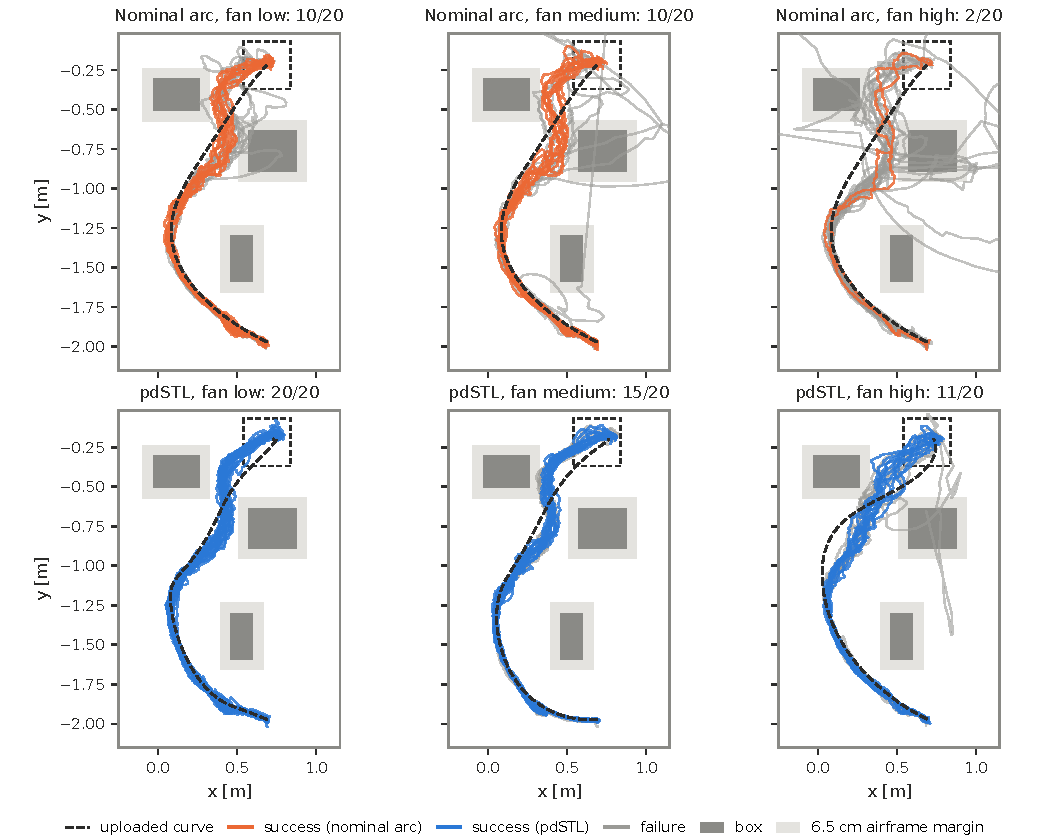
\includegraphics[width=\textwidth]{figures/flown_paths.pdf}
  \caption{Flown paths, first 20 flights per group. Top: nominal arc;
  bottom: pdSTL plan for each fan setting. Coloured paths succeeded, grey
  paths failed. Dark boxes are the measured obstacles, light bands the
  6.5\,cm airframe margin, the dashed square the goal.}
  \label{fig:paths}
\end{figure*}

\begin{figure}[t]
  \centering
  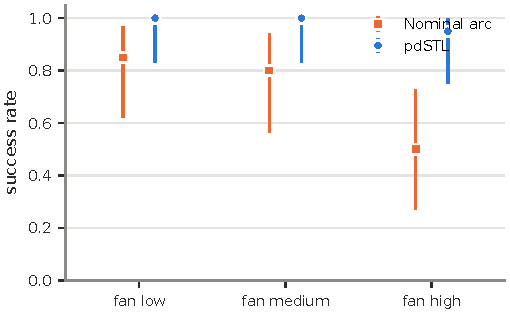
\includegraphics[width=\columnwidth]{figures/success_rates.pdf}
  \caption{Success rate with 95\,\% Clopper--Pearson intervals, 20 flights
  per point.}
  \label{fig:success}
\end{figure}

pdSTL succeeded more often than the nominal arc at every fan setting
(Table~\ref{tab:hw-results}, Fig.~\ref{fig:success}): 20/20 against 10/20
at low, 15/20 against 10/20 at medium, and 11/20 against 2/20 at high.
The difference is significant at low ($p = 0.0002$, Holm-adjusted
$0.0007$) and high ($p = 0.003$, adjusted $0.006$), but not at medium
($p = 0.095$). Over all settings, the odds of success are 8.1 times higher
with pdSTL ($p = 7 \times 10^{-6}$).

The two conditions fail differently (Fig.~\ref{fig:paths}). The nominal
arc is pushed into the middle box at about 9\,s and onto the upper-left
box at about 10.5\,s; at high its centre entered a measured box in 9 of
20 flights. The pdSTL plans mostly fail by grazing the upper-left box
inside the airframe margin; their centre entered a box in 1 of 60 flights.
At medium, pdSTL had no falls (0/20 against 9/20) and held its height in
every flight.

\paragraph{Robustness of the comparison}
The overall result does not depend on the choices made after flying.
With the last 20 flights per group instead of the first, or with every
flight, the stratified test gives an odds ratio of 4.4 ($p = 3 \times
10^{-4}$) and 4.5 ($p = 2 \times 10^{-4}$). With the earlier, more
conservative 7\,cm margin it gives 9.7 ($p = 1 \times 10^{-6}$). The
per-setting results at medium and high are less stable: with every flight
their one-sided $p$ values are 0.25 and 0.026.

\paragraph{Model calibration}
The model is overconfident. It predicts $\Pr(\varphi) \ge 0.988$ for every
pdSTL plan, but the observed rates are 1.00, 0.75 and 0.55. For the
nominal arc it predicts 0.999, 0.985 and 0.566 against 0.50, 0.50 and
0.10. Two effects explain most of the gap. First, the push depends on
where the drone is in the airflow, not only on the time along the path:
at high, the pdSTL flights flew 10--12\,cm left of the predicted mean
near the gap, because the shifted path met a weaker push than the nominal
arc did. Second, the wind changed between days: on the medium evaluation
day the push on the nominal arc reached about 18\,cm at 10.8\,s, against
9.5\,cm two days earlier during identification. In addition, falls and
height loss, which the planar model does not describe, account for many
failures at high.
% TODO(Bennett): your reading of what this means for the method, and
% whether to close the loop (refit on flown plans) as future work.

\subsection{Deviations from the plan}

We report the decisions made after the evaluation flights:
\begin{itemize}
  \item Height was removed from the success measure. The planner does not
    plan height, and in several flights the drone dipped in the gap's
    airflow and recovered. Height and falls are reported beside success.
  \item The airframe radius was changed from 7\,cm to the measured
    propeller-tip radius of 6.5\,cm. The plans were made with 7\,cm and
    are therefore slightly more cautious than the scoring requires.
  \item One box was remeasured and found 3\,cm from its recorded position.
    It stood there during all flights; the record was corrected.
  \item Groups had 20 to 25 flights. The first 20 per group are reported.
\end{itemize}
% TODO(Bennett): decide whether this list goes in the paper, a footnote,
% or the supplementary material.
